\documentclass[11pt,compress,t,notes=noshow, xcolor=table]{beamer}
\input{../../style/preamble_new}
\input{../../latex-math/basic-math.tex}
\input{../../latex-math/basic-ml.tex}

\title{Deep Learning for NLP}

\definecolor{texblue}{rgb}{0, 0, 1}
\def\myblue#1{\textcolor{texblue}{#1}}
\long\def\devour#1{}

\definecolor{texblue}{rgb}{0, 0, 1}
\def\myblue#1{\textcolor{texblue}{#1}}


\begin{document}

%\devour{

\titlemeta{
Training LLMs
}{
How to reduce compute and memory
}{
figure/gpu_mem.png
}{
\item Learn about distributed training with data/tensor parallelism
\item Learn about FlashAttention
}

% ------------------------------------------------------------------------------

\begin{vbframe}{Why Distribute LLM Training?}

Training large models on one GPU has two problems:

\begin{itemize}
    \item \textbf{Speed:} training may take too long.
    \item \textbf{Memory:} the model and training state may not fit.
\end{itemize}

Using several GPUs can address both, but the computation must be
distributed appropriately.

Two basic strategies are:

\begin{itemize}
    \item \textbf{Data parallelism:} replicate the model and split the data.
    \item \textbf{Tensor parallelism:} split the model itself across GPUs.
\end{itemize}

\begin{center}
\textbf{Different strategies solve different bottlenecks.}
\end{center}

\end{vbframe}


\begin{vbframe}{Data Parallelism: Same Model, Different Data}

\begin{columns}[T]
\begin{column}{0.55\textwidth}

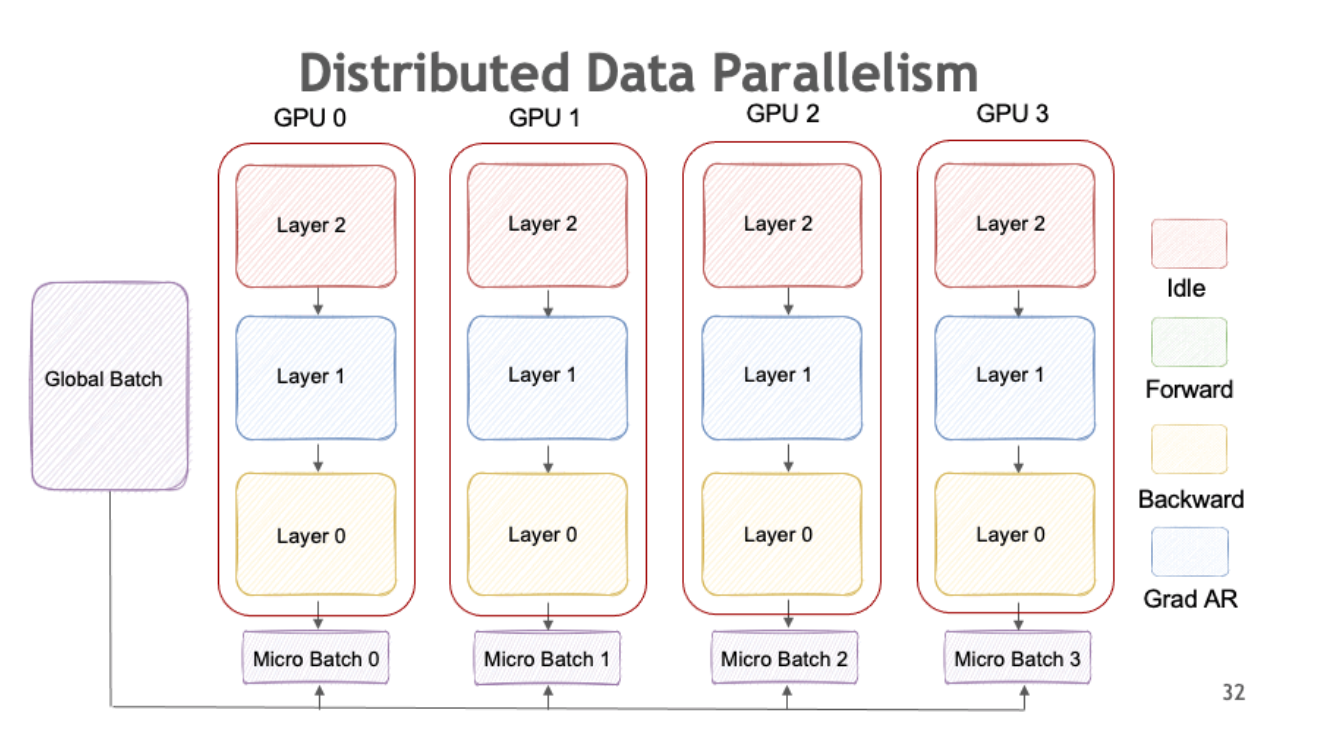
\includegraphics[width=\textwidth]{./figure/data_parallel.png}

{\footnotesize
Source:
\href{https://docs.nvidia.com/nemo-framework/user-guide/latest/nemotoolkit/features/parallelisms.html#distributed-data-parallelism}
{Nvidia}
}

\end{column}

\begin{column}{0.43\textwidth}

Each GPU

\begin{itemize}
    \item stores a \textbf{full copy of the model},
    \item processes a different part of the batch,
    \item computes gradients locally.
\end{itemize}

The gradients are then averaged across GPUs
(\textbf{All Reduce}).

All GPUs apply the same update, so their model copies remain identical.

\end{column}
\end{columns}

\end{vbframe}


% ------------------------------------------------------------------------------

\begin{vbframe}{What Does Data Parallelism Buy Us?}

Different GPUs process different training examples \textbf{in parallel}.

Therefore, data parallelism can increase training throughput:

\[
\text{more GPUs}
\quad\Longrightarrow\quad
\text{more examples processed per second}.
\]

But every GPU still stores the \textbf{entire model}.

\begin{itemize}
    \item Good for reducing training time.
    \item Does \textbf{not} allow a model that is too large for one GPU
          to fit.
    \item Gradient synchronization adds communication overhead.
\end{itemize}

\begin{center}
\textbf{To split the model itself, we need tensor parallelism.}
\end{center}

\end{vbframe}

% ------------------------------------------------------------------------------

\begin{vbframe}{Tensor Parallelism: Split the Model Across GPUs}

\begin{columns}[T]
\begin{column}{0.48\textwidth}

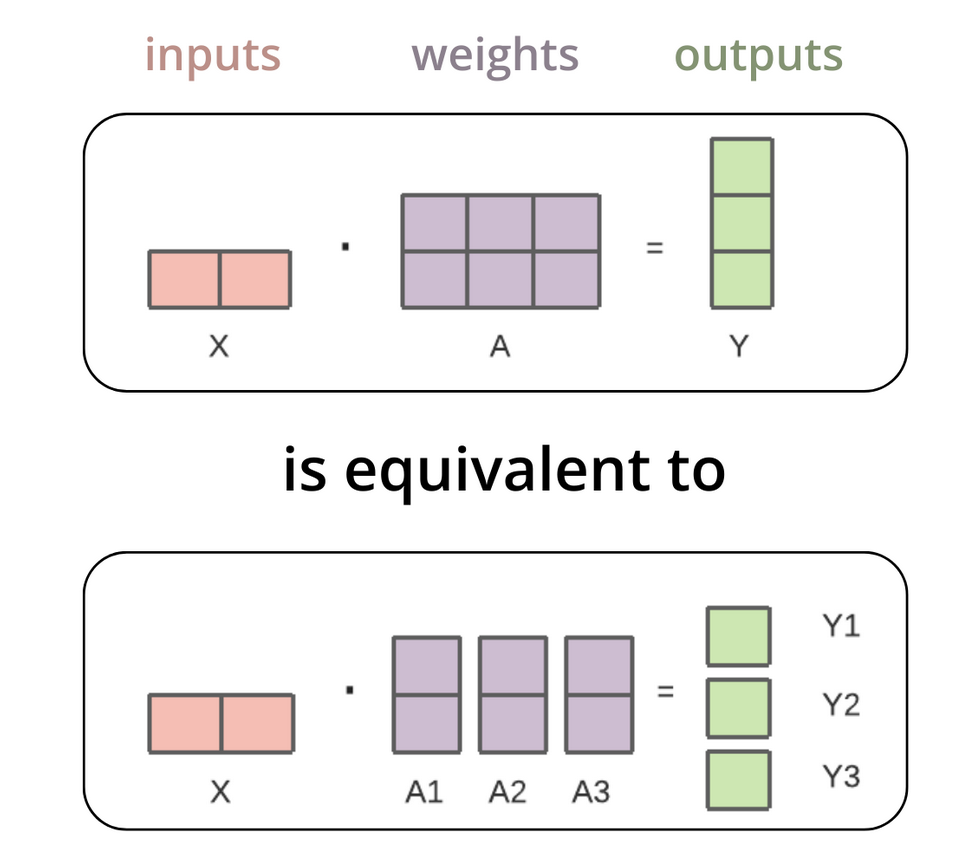
\includegraphics[width=\textwidth]{./figure/tensor,parallelism,new.png}

{\footnotesize
Source:
\href{https://docs.nvidia.com/nemo-framework/user-guide/latest/nemotoolkit/features/parallelisms.html#tensor-parallelism}
{Nvidia}
}

\end{column}

\begin{column}{0.49\textwidth}

Instead of replicating the full model, split large tensors
across GPUs.

For a matrix multiplication

\[
Y = XW,
\]

the weight matrix $W$ can be partitioned across devices.

Each GPU

\begin{itemize}
    \item stores only part of $W$,
    \item computes part of $Y$,
    \item exchanges intermediate results when needed.
\end{itemize}

\end{column}
\end{columns}

\end{vbframe}


% ------------------------------------------------------------------------------

\begin{vbframe}{Data vs.\ Tensor Parallelism}

\[
\begin{array}{l|cc}
 & \textbf{Data parallelism} & \textbf{Tensor parallelism} \\
\hline
\text{Model} & \text{replicated} & \text{split across GPUs} \\
\text{Data} & \text{split} & \text{shared/processed jointly} \\
\text{Main benefit} & \text{higher throughput} & \text{larger models fit} \\
\text{Communication} & \text{between updates} & \text{within layers}
\end{array}
\]

\begin{itemize}
    \item Data parallelism is useful when the model fits on one GPU,
          but training is too slow.
    \item Tensor parallelism is useful when individual model operations
          are too large for one GPU.
\end{itemize}

Large-scale training commonly combines both strategies.

\end{vbframe}


% ------------------------------------------------------------------------------

\begin{vbframe}{Why Is Attention Expensive in Memory?}

For a sequence of $n$ tokens, attention computes

\[
S = QK^\top,
\qquad
P = \operatorname{softmax}(S),
\qquad
O = PV.
\]

Both intermediate matrices contain one value for every pair of tokens:

\[
S,P \in \mathbb{R}^{n\times n}.
\]

Hence, storing them requires

\[
\boxed{O(n^2)\ \text{memory}.}
\]

Doubling the sequence length makes these matrices
about \textbf{4 times larger}.

\begin{center}
\textbf{Can we compute exact attention without storing
these large intermediate matrices?}
\end{center}

\end{vbframe}


% ------------------------------------------------------------------------------

\begin{vbframe}{The GPU Memory Hierarchy}

\begin{columns}[T]

\begin{column}{0.52\textwidth}

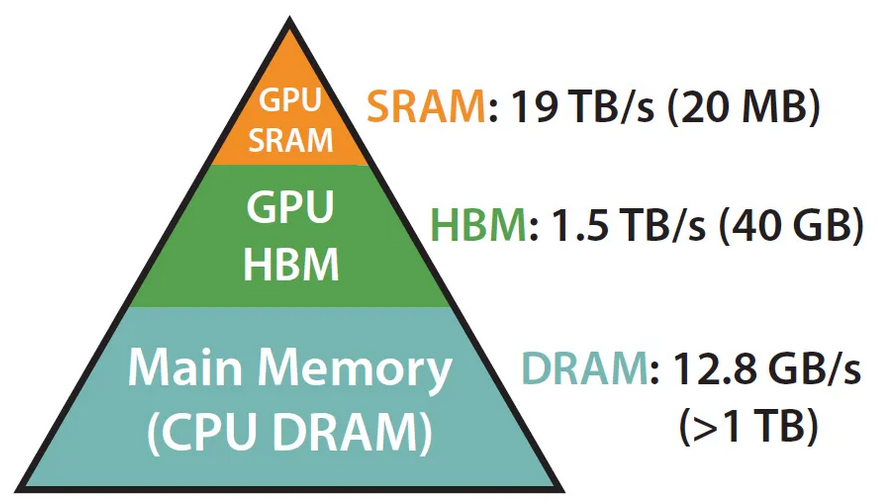
\includegraphics[width=\textwidth]{./figure/gpu_mem.png}

{\footnotesize
\citebutton{Source: Dao et al., 2022}
{https://arxiv.org/abs/2205.14135}
}

\end{column}

\begin{column}{0.45\textwidth}

GPU memory has a hierarchy:

\begin{itemize}
    \item \textbf{Static Random-Access Memory (SRAM):}
          very fast, but small
    \item \textbf{High-Bandwidth Memory (HBM):}
          much larger, but slower
\end{itemize}

GPU compute reads from and writes to SRAM.

Moving data and results between HBM and SRAM
can become the bottleneck.

\begin{center}
\textbf{Reducing this memory traffic can make computation faster.}
\end{center}

\end{column}

\end{columns}

\end{vbframe}


% ------------------------------------------------------------------------------

\begin{vbframe}{Why Standard Attention Moves So Much Data}

A standard GPU implementation typically performs:

\[
Q,K
\;\longrightarrow\;
S=QK^\top
\;\longrightarrow\;
P=\operatorname{softmax}(S)
\;\longrightarrow\;
O=PV.
\]

Between these operations,

\begin{enumerate}
    \item $Q,K$ are read from HBM; $S$ is computed and written to HBM,
    \item $S$ is read back; $P$ is computed and written to HBM,
    \item $P,V$ are read back to compute $O$.
\end{enumerate}

Thus, the large $n\times n$ matrices $S$ and $P$
are repeatedly transferred between HBM and SRAM.

\begin{center}
\textbf{FlashAttention avoids materializing $S$ and $P$ in HBM.}
\end{center}

\citebutton{Dao et al., 2022}
{https://arxiv.org/abs/2205.14135}

\end{vbframe}


% ------------------------------------------------------------------------------

\begin{vbframe}{FlashAttention: Compute Attention Block by Block}

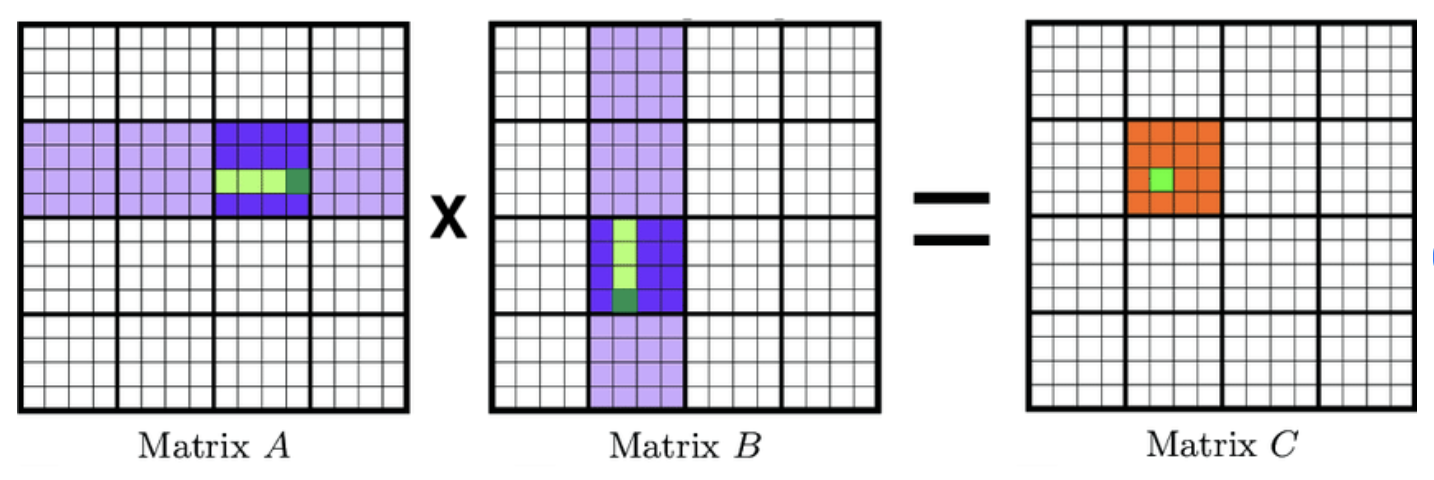
\includegraphics[width=0.6\textwidth]{./figure/tiling}

Take one query block $Q_i$ and process all key/value blocks in turn:

\[
(K_1,V_1),\ (K_2,V_2),\ \ldots
\]

For each block $j$:

\begin{enumerate}
    \item load $Q_i,K_j,V_j$ from HBM into SRAM,
    \item compute $S_{ij}=Q_iK_j^\top$,
    \item update the running softmax normalization,
    \item update the partial output $O_i$, discard $S_{ij}$ and its softmax values.
\end{enumerate}
After the final block, $O_i$ is normalized and written to HBM. All blocks are processed, but not stored at the same time. 

\end{vbframe}


% ------------------------------------------------------------------------------

\begin{vbframe}{FlashAttention: An Illustration}

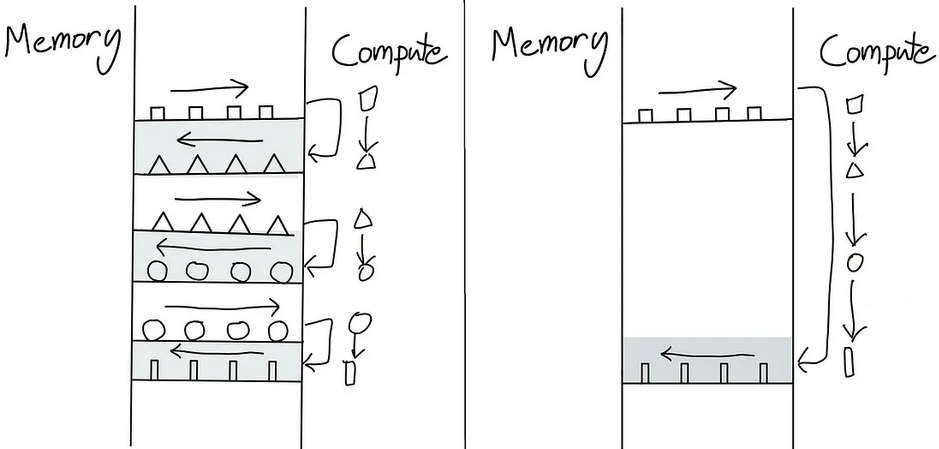
\includegraphics[width=0.6\textwidth]{./figure/op_fusion.png}

{\footnotesize
Source:
\href{https://horace.io/brrr_intro.html}
{horace.io}
}

During the \textbf{forward pass}, each score block $S_{ij}$ and its
softmax probabilities are used and then discarded.

During \textbf{backpropagation}, the same blocks are recomputed from
$Q_i$ and $K_j$ when they are needed again.

\[
\boxed{
\text{more arithmetic}
\;\Longleftrightarrow\;
\text{less memory and HBM traffic}
}
\]

\end{vbframe}

% ------------------------------------------------------------------------------

\begin{vbframe}{Mixture-of-Experts}

FlashAttention makes attention more efficient.
MoE (e.g. Mixtral \citebutton{Jiang et al., 2024: Mixtral}
{https://arxiv.org/abs/2401.04088}) changes the \textbf{feed-forward part} of the Transformer. 

\[
H \rightarrow \text{Self-Attention}
\rightarrow \tilde H
\rightarrow \text{Feed-Forward Network (FFN)}
\rightarrow H'.
\]

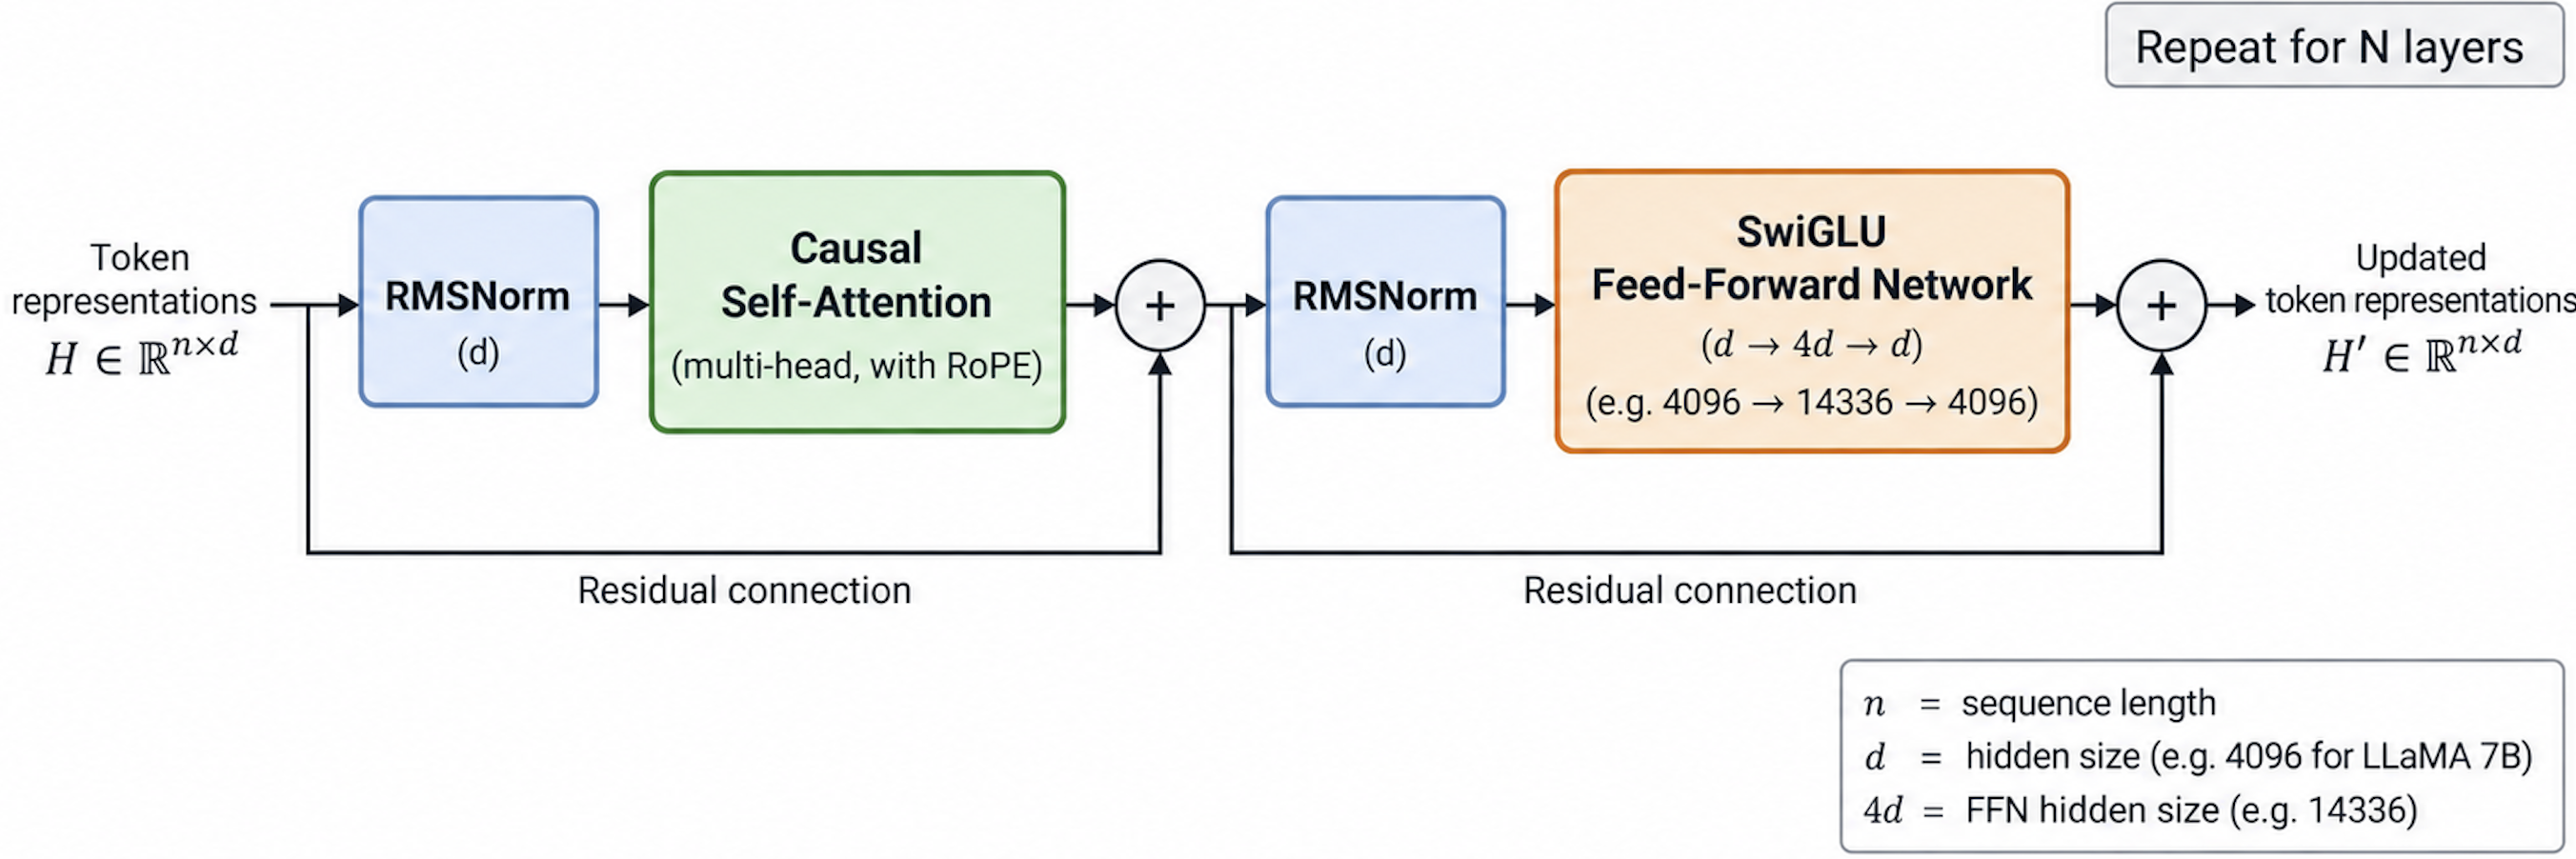
\includegraphics[width=\textwidth]{./figure/llama_transformer_block.png}

\begin{itemize}
    \item Self-attention remains dense.
    \item The single FFN is replaced by 8 \textbf{experts}. (Increase capacity.)
    \item For each token, only 2 experts are evaluated. (But use efficiently.)
\end{itemize}

\end{vbframe}


% ------------------------------------------------------------------------------

\begin{vbframe}{How Does Mixtral Select Experts?}

For each token representation $\tilde h\in\mathbb{R}^{4096}$ after self-attention,
a small router computes 8 scores:

\[
r = W_{\text{router}}\tilde h,
\qquad
W_{\text{router}}\in\mathbb{R}^{8\times4096}.
\]
\begin{itemize}
    \item Select the top 2 experts.
    \item Both process the same token representation $\tilde h$.
    \item Their outputs are weighted and combined.
\end{itemize}
\[
y = w_i E_i(\tilde h) + w_j E_j(\tilde h).
\]
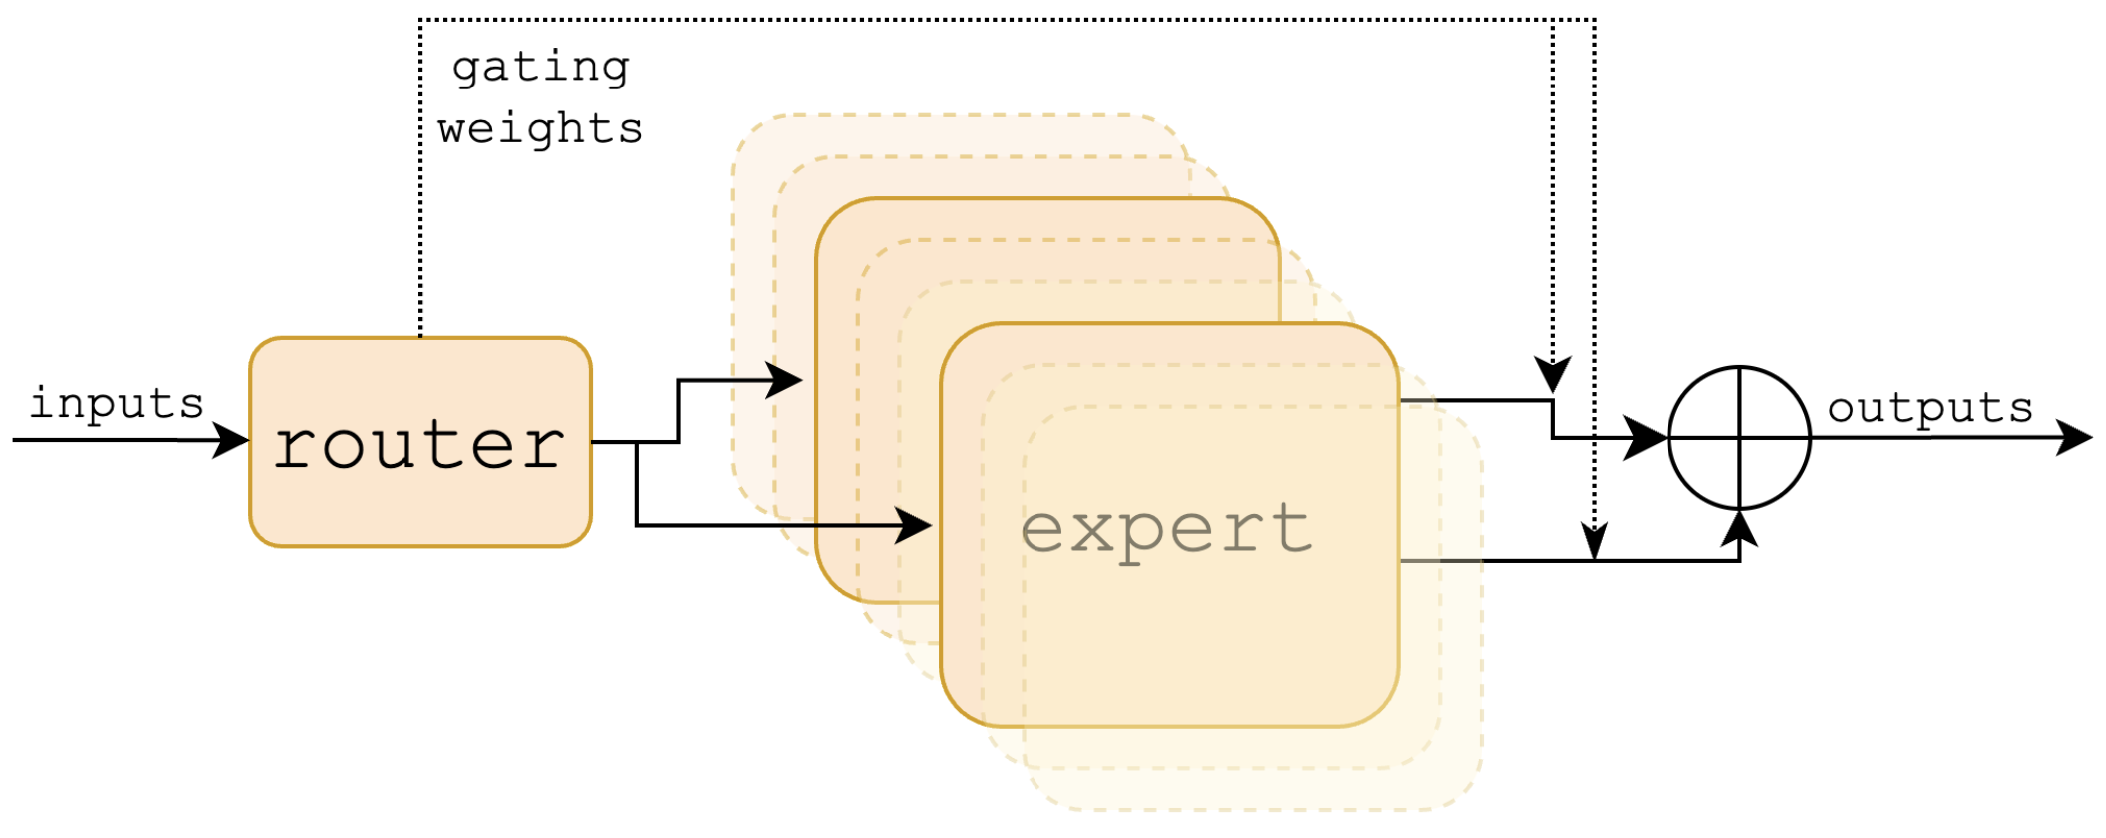
\includegraphics[width=0.65\textwidth]{./figure/mixtral_experts.png}

%\citebutton{Jiang et al., 2024: Mixtral}
%{https://arxiv.org/abs/2401.04088}

\end{vbframe}


% ------------------------------------------------------------------------------

\begin{vbframe}{Sparse Routing Saves Compute}

Each expert in Mixtral is a full SwiGLU FFN:

\[
4096 \rightarrow 14336 \rightarrow 4096.
\]

It has three projection matrices (including a gating projection):
\citebutton{Shazeer, 2020}
{https://arxiv.org/abs/2002.05202}
\[
P_{\text{expert}}
\approx 3\cdot4096\cdot14336
\approx176\text{M}.
\]

Mixtral stores 8 experts, but evaluates only 2 per token:

\[
8\times176\text{M stored}
\qquad\text{vs.}\qquad
2\times176\text{M evaluated}.
\]

(The router adds only about $8\cdot4096\approx33{,}000$
parameters.)

Across the model:

\[
\boxed{47\text{B total parameters} \qquad \approx13\text{B active/token}}
\]

\begin{center}
\textbf{More capacity without activating all parameters for every token.}
\end{center}

\end{vbframe}



\endlecture
\end{document}

% ------------------------------------------------------------------------------

